\chapter{基礎概念}
\label{chap:concept}

\section{緒言}
船舶の運行状況予測をするにあたり、予測に使用した学習モデルや評価指標について述べる。

\section{CNN}
CNNとは畳み込みニューラルネットワークのことで畳み込み層やプーリング層などの層が積み重なったニューラルネットワークであり、
Y. LeCun\cite{Yann LeCun}らが最初に提唱した畳み込みニューラルネットワーク図\ref{lenet}が有名である。
画像を入力とした畳み込みニューラルネットワークの特徴的な層について説明する。
\begin{figure}[H]
 \centering
 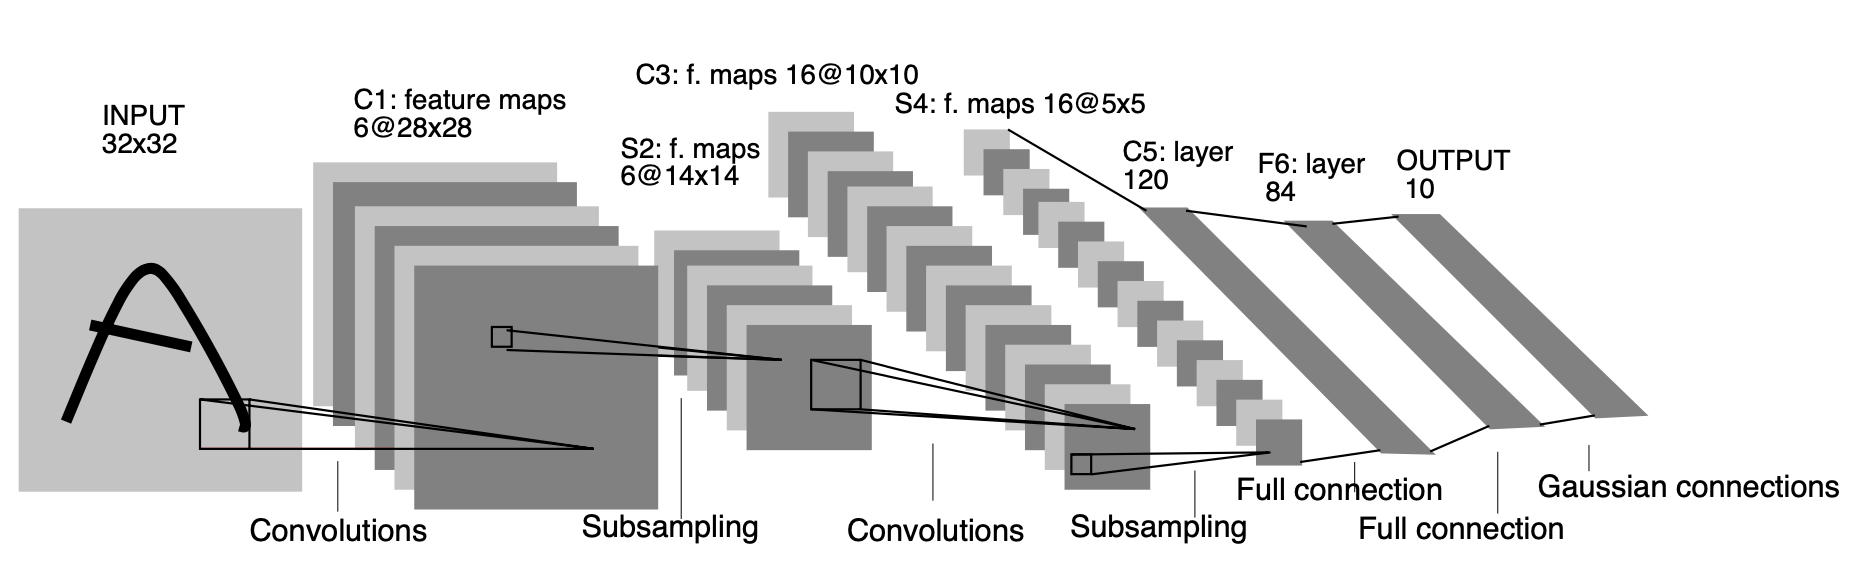
\includegraphics[keepaspectratio, scale=0.5]{fig/chapter2/Lenet-5.png}
 \caption{CNNの例\cite{Yann LeCun}}
 \label{lenet}
\end{figure}
\subsection{畳み込み層}
入力画像を畳み込み層に入力し画像から特徴を図\ref{tatami}にのように抽出する。
図\ref{tatami}では入力画像がカラー画像(RGB)の場合、入力に対してR、G、Bそれぞれのチャンネルに対して対応するフィルタを適用する。R、G、Bの入力に対してフィルタを重ね合わせ、合わせた部分の画素値に乗算を適用し合計値を算出、さらにR、G、Bの合計値により出力の画素値が決定し、その処理をスライドさせながら画像全体に対して行う。
\begin{figure}[H]
 \centering
 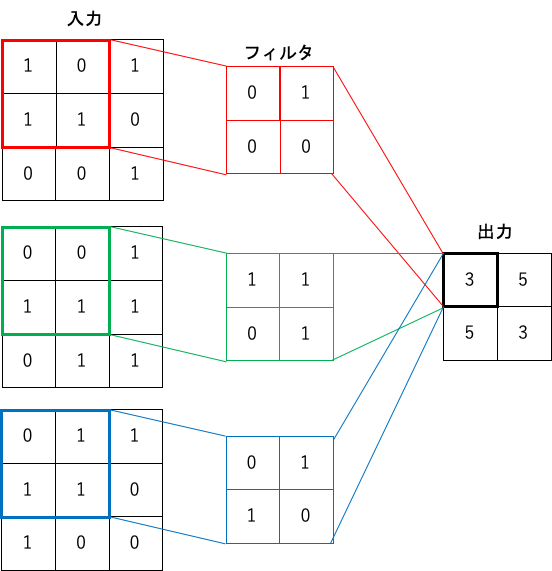
\includegraphics[keepaspectratio, scale=0.4]{fig/chapter2/tatamikomi.png}
 \caption{畳み込み層の出力例}
 \label{tatami}
\end{figure}

\subsection{プリーング層}
プーリング層とは入力画像内の局所的な情報を集めることである。とくにMax Poolingの図\ref{pooling}では入力に対して局所的な領域の最大値を出力する処理を行うことである。

\begin{figure}[H]
 \centering
 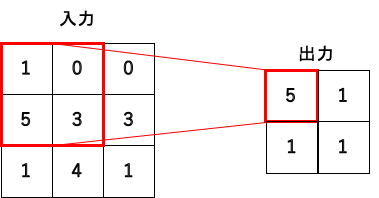
\includegraphics[keepaspectratio, scale=0.5]{fig/chapter2/pooling.png}
 \caption{プーリング層の出力例}
 \label{pooling}
\end{figure}


\section{LightGBM}
LightGBMとは決定木アルゴリズムをベースにした勾配ブースティングの機械学習フレームワークである。LightGBMの特徴として決定木、アンサンブル学習、勾配ブースティングなどがある。それぞれについて説明する。
\subsection{決定木}
LightGBMでは決定木を基にしたアルゴリズムを使用している。決定木とは図\ref{kettei}のように項目において閾値を決定し閾値により条件分岐させ木のように成長させて問題を解くアルゴリズムである。
\begin{figure}[H]
 \centering
 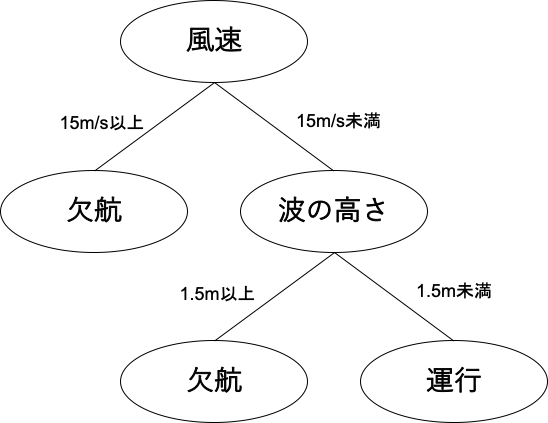
\includegraphics[keepaspectratio, scale=0.6]{fig/chapter2/ketteigi.png}
 \caption{決定木の例}
 \label{kettei}
\end{figure}

\subsection{アンサンブル学習}
アンサンブル学習とは複数のモデルを学習させて1つの学習モデルを生み出す学種方法である。このようにすることで精度の低いモデルでも高精度な予測をすることができる。図\ref{ensemble}の例ではモデルの数を4つとしたときにそれぞれのモデルの予測結果の多数決をとることで最終的に100%の精度で予測することができる。
\begin{figure}[H]
 \centering
 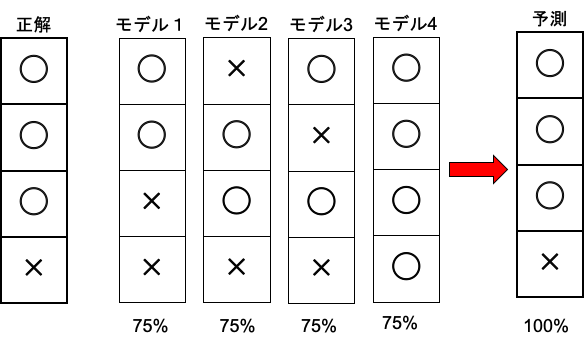
\includegraphics[keepaspectratio, scale=0.4]{fig/chapter2/ensemble.png}
 \caption{アンサンブルの例}
 \label{ensemble}
\end{figure}

\subsection{勾配ブースティング}
勾配ブースティングはアンサンブル学習の手法のひとつである。ブースティングとはデータセットの中から一部のデータを用いてモデルを学習し評価を行う。その後の別モデルで前のモデルで誤った予測をしたデータを学習し評価を行いさらに次のモデルでも同じことを行うことでデータの誤差の学習を行う。最後に各モデルの多数決を行いモデルを組み合わせる。

\section{windy.com}
本研究に使用したデータを取得してきたwebサイトである。このサイトは世界中の天気予報を可視化でき、リアルタイムの気象状況や気象値、数日先までの予報を閲覧することができる。レイヤー機能があり風速レイヤー、波高レイヤーや気温レイヤーなど様々なレイヤーを使用でき、レイヤーごとの特徴を視覚的に見ることができる\cite{windy}。

\section{安栄観光}
本研究に使用した教師データを取得してきたwebサイトである。このサイトでは主に石垣島から西表島への7つある航路の船舶運行状況を確認できる\cite{anei}。


\section{予測精度の評価指標}
本研究では上記で説明した学習モデルで入力を画像とする場合はCNNを採用し、数値を入力する場合はLightGBMを採用する。予報図(画像)、気象状況(数値)の比較を行うためそれぞれの予測精度を評価する必要がある。本研究の問題は二値分類問題であるので一般に正解率、適合率、再現率、F値を使用して評価をすることが多い。そのため本研究でもこれらの評価指標を用いて評価を行なう。%本節ではこれらの評価指標の説明を行う。

%\subsection{正解率}


